% ============================================================================
% EXERCISE 1 (Steps 1-3): el codigo MC, sin serie en densidad
% RESPONSABLE: Torret (toda la seccion)
% ============================================================================
\section{Part 1 (Steps 1--3)}

\subsection{Question}
Determine the equation of state of a Lennard-Jones fluid for the isotherm $T^*=2.0$ with a personal Monte Carlo code ($N\sim 500$ atoms):
\begin{enumerate}
  \item Write a MC code for an $(N,V,T)$ simulation of a Lennard-Jones system, using \texttt{leapfroglj.f} as the starting point.
  \item Compute the interaction energy $U=\langle\sum_i\sum_{j>i}U(r_{ij})\rangle$ and the pressure $P=\rho k_BT+\frac{1}{3V}\langle\sum_i\sum_{j>i}\vec r_{ij}\cdot\vec F_{ij}\rangle$, with their standard deviations $\sigma_U$ and $\sigma_P$.
  \item Compute the radial distribution function $g(r)$.
\end{enumerate}

\subsection{Code}
First of all, we adapted the \texttt{mcnvt.f90} was built from \texttt{leapfroglj.f90} (Practice~2). It works in reduced units ($\sigma=\epsilon=k_B=1$), with $N=500$ atoms in a cubic box with periodic boundary conditions (minimum image) and a Lennard-Jones potential truncated at $r_c=2.5\sigma$. The full program is in the Annex; the key pieces are below.

One Metropolis trial move (Step~1): a random atom is displaced by up to $\pm\Delta/2$ along each axis and accepted with probability $\min\{1,e^{-\beta\,\delta U}\}$. Only the energy of the moved atom with the others is computed ($O(N)$ per move).
\lstinputlisting[style=fortranstyle,firstline=306,lastline=344,firstnumber=306,caption={Metropolis move \texttt{mcmove}.},label={lst:mcmove}]{../mcnvt.f90}

Energy, virial and $g(r)$ histogram are evaluated on the whole configuration every \texttt{nsamp} moves (Steps~2--3). The tail corrections for a uniform fluid beyond $r_c$ are added to $U$ and $P$,
\begin{equation}
  \frac{U_{\mathrm{tail}}}{N}=\frac{8\pi}{3}\rho\Big(\frac{1}{3r_c^9}-\frac{1}{r_c^3}\Big),\qquad
  P_{\mathrm{tail}}=\frac{16\pi}{3}\rho^2\Big(\frac{2}{3r_c^9}-\frac{1}{r_c^3}\Big).
\end{equation}
\lstinputlisting[style=fortranstyle,firstline=61,lastline=65,firstnumber=61,caption={Tail corrections.},label={lst:tail}]{../mcnvt.f90}
\lstinputlisting[style=fortranstyle,firstline=169,lastline=191,firstnumber=169,caption={Subroutine \texttt{sample}: $U$ and $P$ (virial route) of the current configuration.},label={lst:sample}]{../mcnvt.f90}

$\sigma_U$ and $\sigma_P$ are the standard deviations of the values sampled along the run (2000 samples per run).

\subsection{Results}
Figure~\ref{fig:traces} shows the output of one run of the program (the $\rho^*=0.5$ point of the series of Part~2, $10^7$ moves, starting from an fcc lattice): the sampled $U^*/N$ and $P^*$ and their running means. The run gives $U^*/N=-3.152$, $\sigma_U=0.051$, $P^*=1.067$, $\sigma_P=0.154$, with an acceptance rate of $46\%$ ($\Delta^*=0.527$). The $g(r)$ of the same run is in Figure~\ref{fig:gdr}.

\begin{figure}[H]
  \centering
  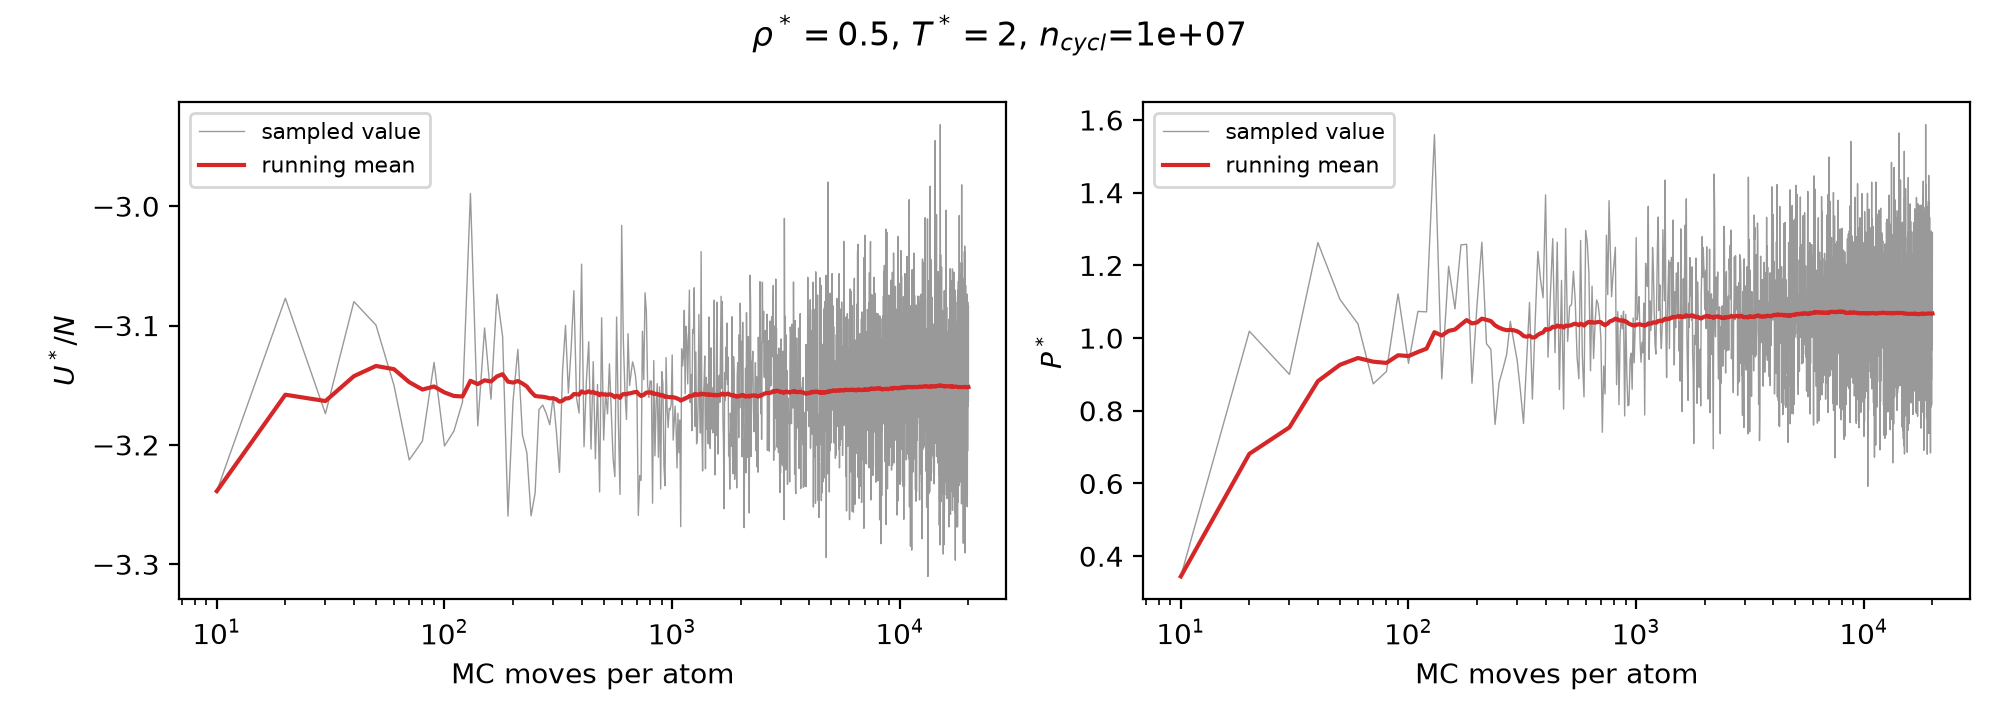
\includegraphics[width=\linewidth]{../figures/traces_rho05.png}
  \caption{Sampled $U^*/N$ (left) and $P^*$ (right) along one MC run at $\rho^*=0.5$, $T^*=2.0$ (one sample every $10$ moves per atom), with their running means. Logarithmic horizontal axis.}
  \label{fig:traces}
\end{figure}

\subsection{Discussion \& Notes}
\begin{itemize}
  \item \textbf{Metropolis move.} Since only one atom moves, $\delta U$ needs only its $N-1$ pairs, so a trial move costs $O(N)$ instead of the $O(N^2)$ of a full evaluation. The full sums (energy, virial, $g(r)$) are done only every \texttt{nsamp} moves.

  \item \textbf{Equilibration.} The run starts from an fcc lattice, but the first sample (after $10$ moves per atom) is already at $U^*/N=-3.24$, close to the mean $-3.15$: the lattice melts almost at once at $T^*=2$. The running mean of $U$ is flat after $\sim\!10^2$ moves per atom and that of $P$ after $\sim\!10^3$, out of $2\times10^4$, so no initial cycles were discarded.

  \item \textbf{Tail corrections.} With $r_c=2.5\sigma$ they are not negligible: $-0.27$ in $P^*$ at $\rho^*=0.5$, a quarter of the total pressure. They assume $g(r)=1$ beyond $r_c$, which is checked in Part~2.

  \item \textbf{Meaning of $\sigma_U$, $\sigma_P$.} They are the fluctuations of the instantaneous values (the width of the grey band in Figure~\ref{fig:traces}), not the error of the mean, which is much smaller because the $2000$ samples are averaged. $\sigma_P$ is about nine times larger than $\sigma_U$ in relative terms ($14\%$ vs $1.6\%$): the virial is dominated by the steep repulsive part of the potential, very sensitive to close pairs.
\end{itemize}

% ============================================================================
% EXERCISE 2 (Steps 4-7): serie en densidad rho* = 0.1-0.8
% RESPONSABLE: Montull, salvo los puntos de Discussion marcados Torret
% ============================================================================
\newpage
\section{Part 2 (Steps 4--7)}

\subsection{Question}
\begin{enumerate}
  \setcounter{enumi}{3}
  \item Perform a series of MC simulations at $T^*=2.0$ and densities from $\rho^*=0.1$ to $0.8$, with $n_{\mathrm{cycl}}\sim10^6,10^7$. List the technical parameters (number of cycles, displacement $\Delta$, acceptance rate, cutoff $r_c$) and the results ($U,\sigma_U,P,\sigma_P$).
  \item Plot $U^*$ and $P^*$ as a function of $\rho^*$. Up to what density is the ideal gas law $P=\rho k_BT$ a good approximation?
  \item Plot $g(r)$ for the different densities.
  \item Obtain $U$ and $P$ by numerical integration of $g(r)$,
  \begin{equation}
    U=2\pi\rho N\!\int_0^\infty\! U(r)g(r)r^2dr,\qquad P=\rho k_BT-\frac{2\pi}{3}\rho^2\!\int_0^\infty\!\frac{dU(r)}{dr}g(r)r^3dr,
  \end{equation}
  and compare with the direct results of Step~4.
\end{enumerate}

\subsection{Code}
The program of Part~1 is used unchanged. The series (Step~4) is launched by \texttt{run\_series.py}: it builds an fcc lattice of $500$ atoms at each $\rho^*$, tunes $\Delta$ with short runs for an acceptance rate near $50\%$ (for $\rho^*\le0.3$ the acceptance stays higher, $\Delta^*=0.881$), and then runs the production. Step~7 was done with \texttt{integrar\_gdr.py}, which integrates the saved $g(r)$ (500 bins up to $L/2$) up to $r_c$ with the rectangle rule and adds the same tail corrections. Figures are made by \texttt{plot\_eos.py}.

\subsection{Results}
Tables~\ref{tab:n1000000} and~\ref{tab:n10000000} list the technical parameters and the results of the two series ($n_{\mathrm{cycl}}=10^6$ and $10^7$ moves, i.e.\ $2000$ and $20000$ moves per atom; cutoff $r_c^*=2.5$).

\begin{table}[H]\centering\small
\caption{Technical parameters and results for $n_{\mathrm{cycl}}=10^6$ ($N=500$, $T^*=2.0$, $r_c^*=2.5$). $\sigma_U$ and $\sigma_P$ are the standard deviations of the sampled values (2000 samples per run, one every $n_{\mathrm{cycl}}/2000$ moves). $U$ is per atom and includes the tail correction.}
\label{tab:n1000000}
\begin{tabular}{ccccccc}\hline
$\rho^*$ & $\Delta^*$ & acc.\ (\%) & $U^*/N$ & $\sigma_U$ & $P^*$ & $\sigma_P$ \\ \hline
0.1 & 0.881 & 77.3 & -0.6571 & 0.035 & 0.1774 & 0.013 \\
0.2 & 0.881 & 61.8 & -1.3091 & 0.043 & 0.3306 & 0.037 \\
0.3 & 0.881 & 49.4 & -1.9217 & 0.046 & 0.4854 & 0.068 \\
0.4 & 0.666 & 47.7 & -2.5357 & 0.047 & 0.6958 & 0.118 \\
0.5 & 0.527 & 46.0 & -3.1540 & 0.049 & 1.0642 & 0.172 \\
0.6 & 0.393 & 48.1 & -3.7522 & 0.065 & 1.7310 & 0.269 \\
0.7 & 0.342 & 44.7 & -4.3099 & 0.085 & 2.9960 & 0.388 \\
0.8 & 0.290 & 43.1 & -4.7791 & 0.128 & 5.1621 & 0.615 \\
\hline\end{tabular}\end{table}
\begin{table}[H]\centering\small
\caption{Technical parameters and results for $n_{\mathrm{cycl}}=10^7$ ($N=500$, $T^*=2.0$, $r_c^*=2.5$). $\sigma_U$ and $\sigma_P$ are the standard deviations of the sampled values (2000 samples per run, one every $n_{\mathrm{cycl}}/2000$ moves). $U$ is per atom and includes the tail correction.}
\label{tab:n10000000}
\begin{tabular}{ccccccc}\hline
$\rho^*$ & $\Delta^*$ & acc.\ (\%) & $U^*/N$ & $\sigma_U$ & $P^*$ & $\sigma_P$ \\ \hline
0.1 & 0.881 & 77.1 & -0.6644 & 0.029 & 0.1777 & 0.013 \\
0.2 & 0.881 & 61.7 & -1.3064 & 0.037 & 0.3294 & 0.038 \\
0.3 & 0.881 & 49.4 & -1.9245 & 0.043 & 0.4893 & 0.070 \\
0.4 & 0.666 & 47.5 & -2.5384 & 0.046 & 0.7045 & 0.110 \\
0.5 & 0.527 & 46.1 & -3.1516 & 0.051 & 1.0673 & 0.154 \\
0.6 & 0.393 & 47.9 & -3.7529 & 0.056 & 1.7403 & 0.204 \\
0.7 & 0.342 & 44.6 & -4.3057 & 0.067 & 3.0182 & 0.279 \\
0.8 & 0.290 & 42.8 & -4.7612 & 0.079 & 5.2534 & 0.353 \\
\hline\end{tabular}\end{table}
\begin{table}[H]\centering\small
\caption{Direct averages (Step~4, $n_{\mathrm{cycl}}=10^7$) against numerical integration of $g(r)$ (Step~7), both with tail corrections.}
\label{tab:integral}\begin{tabular}{ccccccc}\hline
$\rho^*$ & $U_{\mathrm{dir}}$ & $U_{\mathrm{int}}$ & $\Delta U$ & $P_{\mathrm{dir}}$ & $P_{\mathrm{int}}$ & $\Delta P$ \\ \hline
0.1 & -0.6644 & -0.6639 & +0.0006 & 0.1777 & 0.1780 & +0.0003 \\
0.2 & -1.3064 & -1.3058 & +0.0006 & 0.3294 & 0.3301 & +0.0007 \\
0.3 & -1.9245 & -1.9235 & +0.0010 & 0.4893 & 0.4910 & +0.0017 \\
0.4 & -2.5384 & -2.5375 & +0.0010 & 0.7045 & 0.7066 & +0.0021 \\
0.5 & -3.1516 & -3.1504 & +0.0012 & 1.0673 & 1.0706 & +0.0033 \\
0.6 & -3.7529 & -3.7516 & +0.0013 & 1.7403 & 1.7443 & +0.0040 \\
0.7 & -4.3057 & -4.3041 & +0.0017 & 3.0182 & 3.0243 & +0.0061 \\
0.8 & -4.7612 & -4.7592 & +0.0020 & 5.2534 & 5.2614 & +0.0080 \\
\hline\end{tabular}\end{table}
\begin{table}[H]\centering\small
\caption{Comparison with Johnson, Zollweg and Gubbins (1993) at $T^*=2.0$ ($10^7$ cycles; their $r_c$ is $5\sigma$ to $4.27\sigma$, ours $2.5\sigma$ plus tail). The number in parentheses is the error in the last digit(s).}
\label{tab:johnson}\begin{tabular}{cccccc}\hline
$\rho^*$ & $P^*$ (this work) & $P^*$ (Johnson) & $U^*/N$ (this work) & $U^*/N$ (Johnson) & $\Delta P/P$ (\%) \\ \hline
0.1 & 0.1777 & 0.1777(2) & -0.6644 & -0.667(1) & -0.0 \\
0.2 & 0.3294 & 0.3290(6) & -1.3064 & -1.306(1) & +0.1 \\
0.3 & 0.4893 & --- & -1.9245 & --- & --- \\
0.4 & 0.7045 & 0.705(1) & -2.5384 & -2.538(2) & -0.1 \\
0.5 & 1.0673 & 1.069(3) & -3.1516 & -3.149(2) & -0.2 \\
0.6 & 1.7403 & 1.756(7) & -3.7529 & -3.746(2) & -0.9 \\
0.7 & 3.0182 & 3.024(7) & -4.3057 & -4.300(2) & -0.2 \\
0.8 & 5.2534 & 5.28(1) & -4.7612 & -4.753(3) & -0.5 \\
\hline\end{tabular}\end{table}
\begin{table}[H]\centering\small
\caption{Ideal-gas test at $T^*=2.0$ ($10^7$ cycles): compressibility factor $Z=P^*/(\rho^*T^*)$; $Z=1$ for an ideal gas.}
\label{tab:ideal}\begin{tabular}{cccc}\hline $\rho^*$ & $\rho^*T^*$ & $P^*$ & $Z$ \\ \hline
0.1 & 0.20 & 0.1777 & 0.888 \\
0.2 & 0.40 & 0.3294 & 0.823 \\
0.3 & 0.60 & 0.4893 & 0.816 \\
0.4 & 0.80 & 0.7045 & 0.881 \\
0.5 & 1.00 & 1.0673 & 1.067 \\
0.6 & 1.20 & 1.7403 & 1.450 \\
0.7 & 1.40 & 3.0182 & 2.156 \\
0.8 & 1.60 & 5.2534 & 3.283 \\
\hline\end{tabular}\end{table}

\begin{figure}[H]
  \centering
  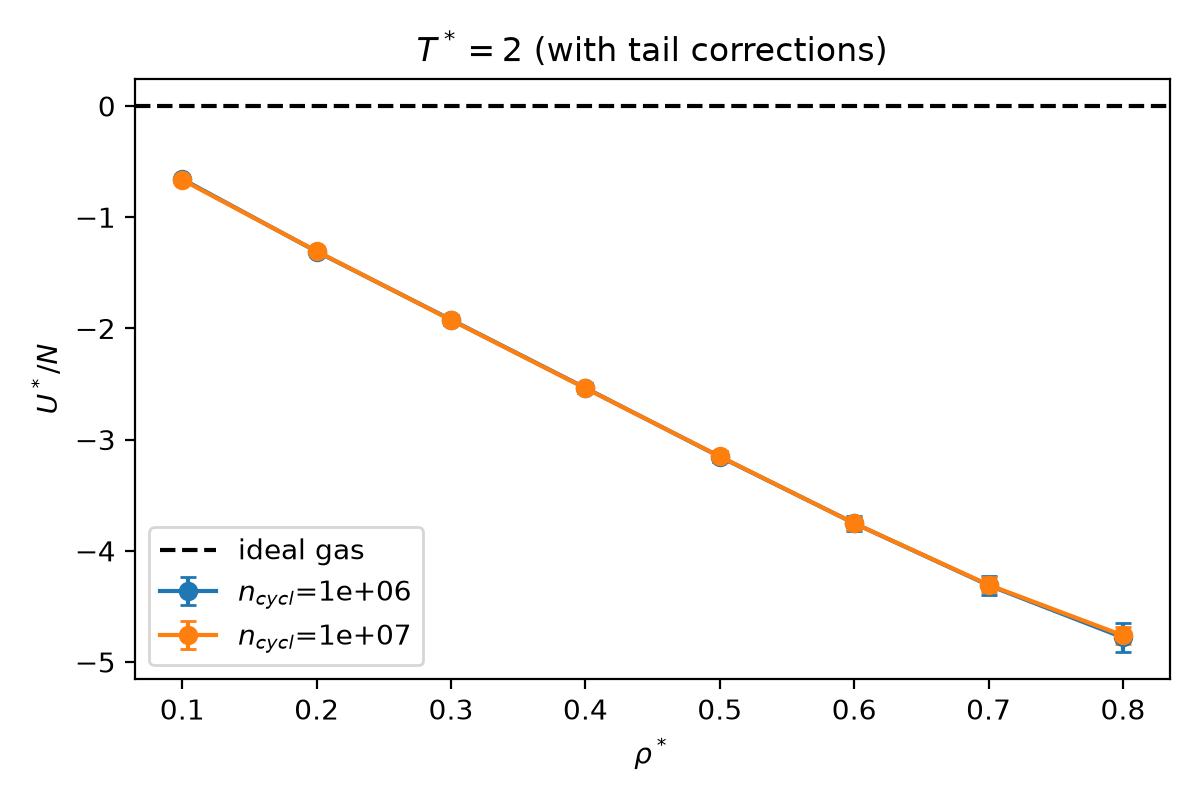
\includegraphics[width=0.48\linewidth]{../figures/U_vs_rho.png}\hfill
  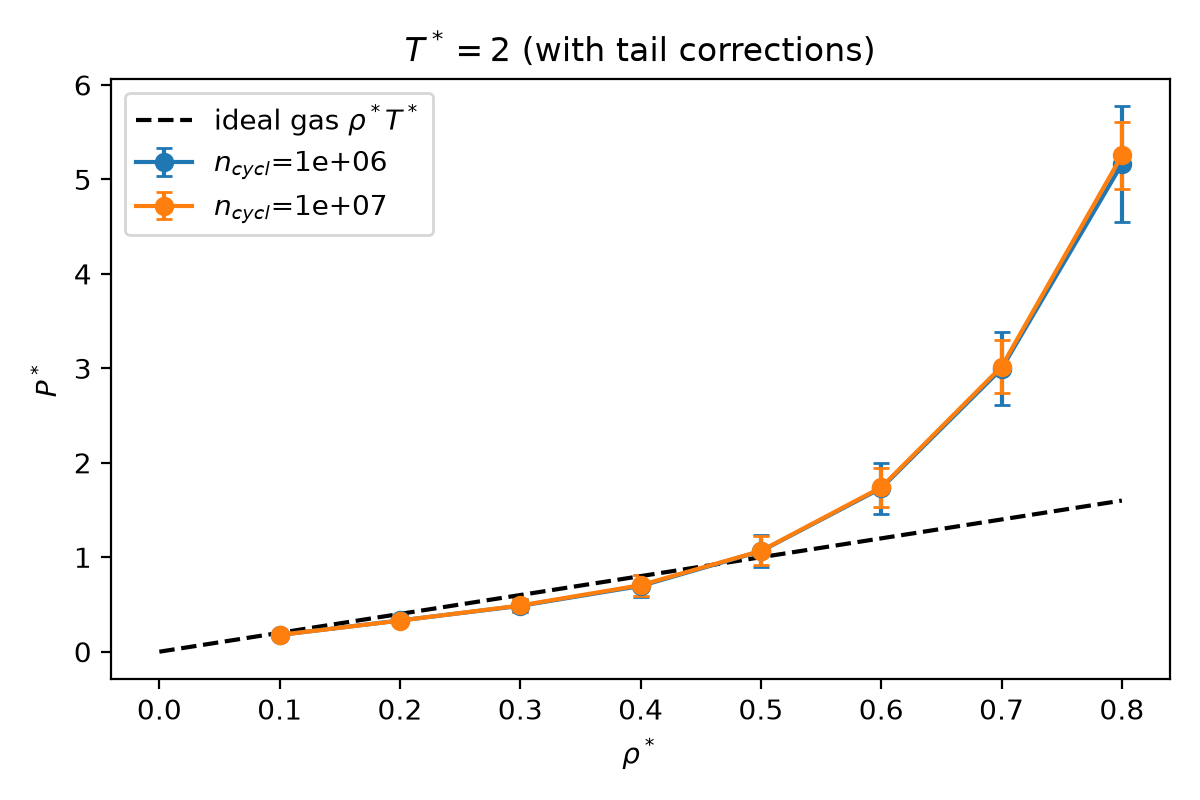
\includegraphics[width=0.48\linewidth]{../figures/P_vs_rho.png}
  \caption{$U^*/N$ (left) and $P^*$ (right) as a function of $\rho^*$ at $T^*=2.0$ for both series; error bars are $\sigma_U$ and $\sigma_P$. The dashed line of the right panel is the ideal gas $P^*=\rho^*T^*$.}
  \label{fig:eos}
\end{figure}

\begin{figure}[H]
  \centering
  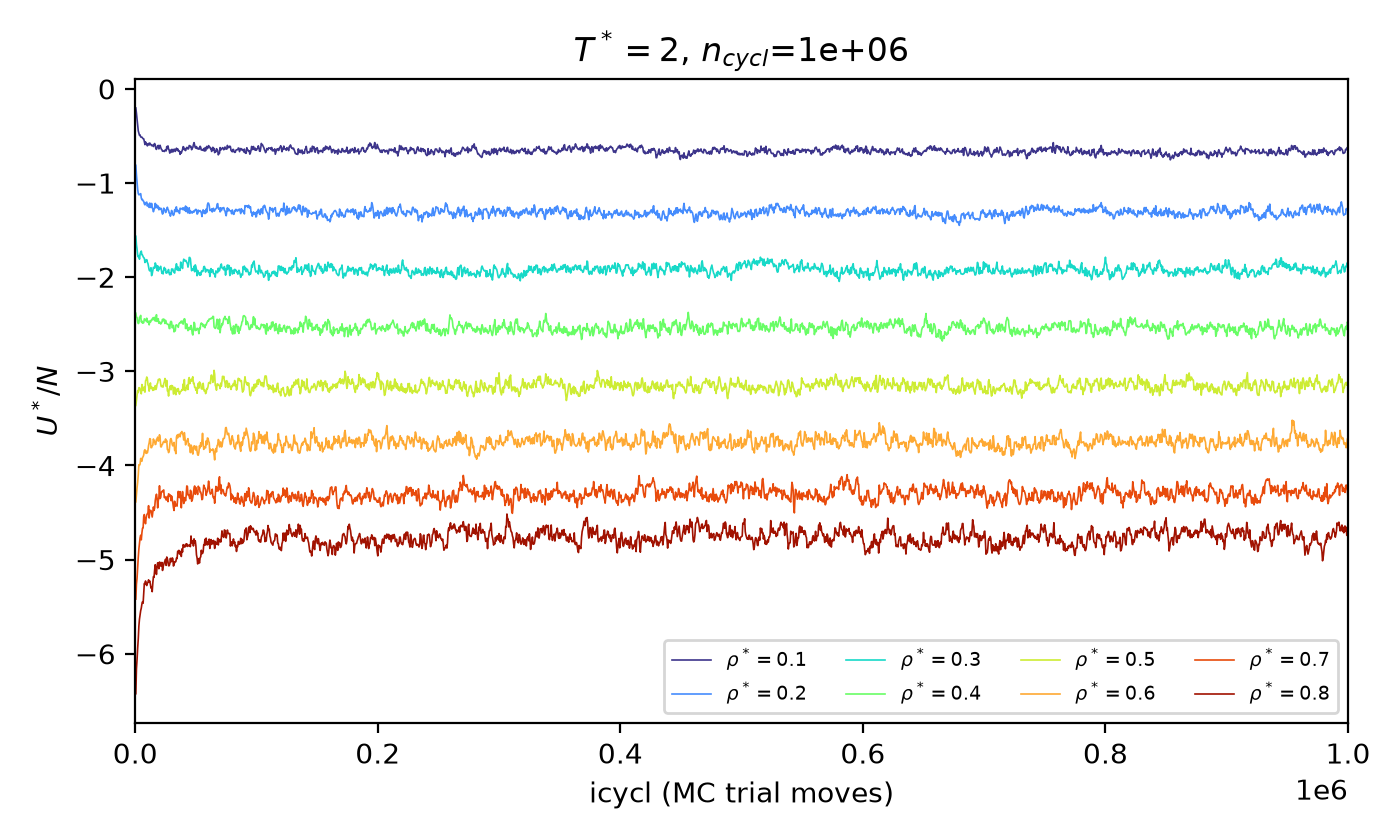
\includegraphics[width=0.8\linewidth]{../figures/U_vs_icycl.png}
  \caption{Sampled $U^*/N$ as a function of the MC move counter \texttt{icycl} for all densities ($T^*=2.0$, $n_{\mathrm{cycl}}=10^6$, fcc start).}
  \label{fig:uicycl}
\end{figure}

\begin{figure}[H]
  \centering
  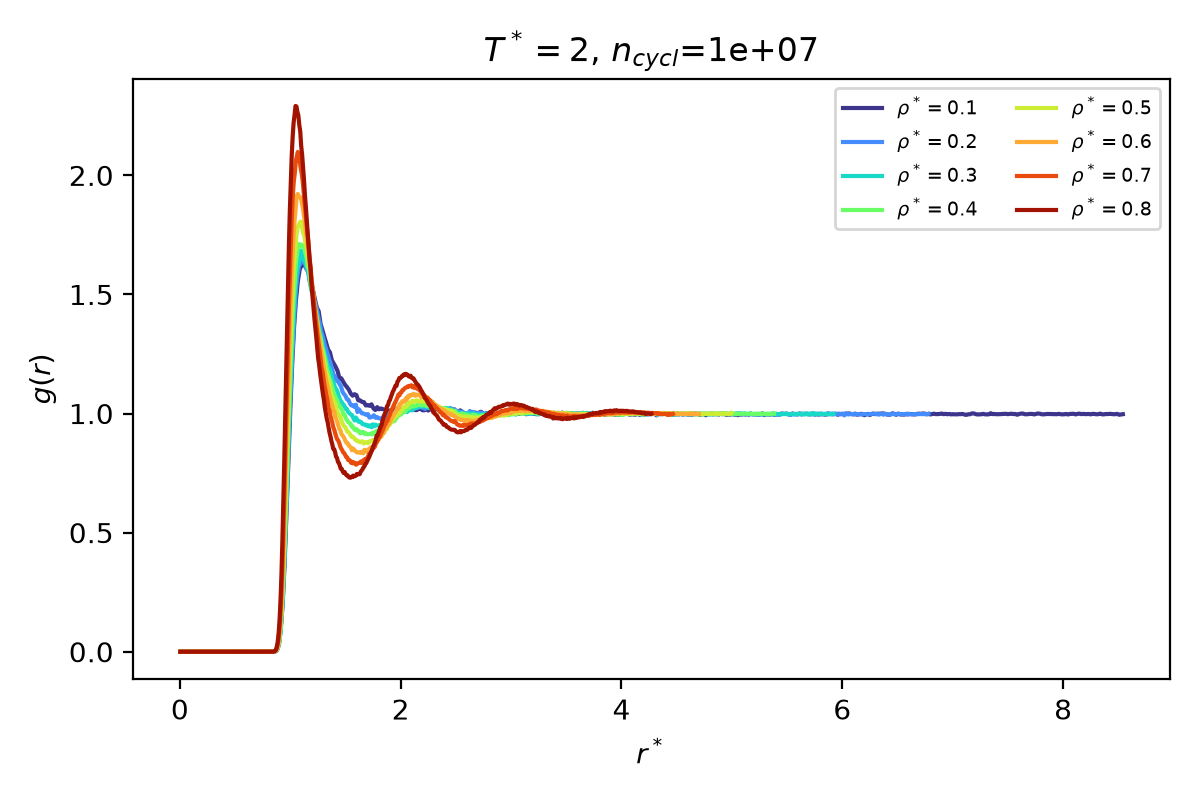
\includegraphics[width=0.7\linewidth]{../figures/gdr.png}
  \caption{Radial distribution function $g(r)$ for $\rho^*=0.1$--$0.8$ ($T^*=2.0$, $10^7$ cycles).}
  \label{fig:gdr}
\end{figure}

\clearpage
\subsection{Discussion \& Notes}
\begin{itemize}
  % RESPONSABLE: Torret
  \item \textbf{Technical parameters.} $\Delta^*$ was tuned so that the acceptance rate is $43$--$48\%$ for $\rho^*\ge0.4$. At low density almost every move is accepted ($77\%$ at $\rho^*=0.1$) because atoms rarely meet; there $\Delta$ is not critical. The cutoff $r_c=2.5\sigma$ is shorter than the $4$--$5\sigma$ of the reference work, which is compensated with the tail corrections. $\sigma_U$ and $\sigma_P$ grow with $\rho^*$ because the dense fluid has large virial fluctuations, and they hardly depend on $n_{\mathrm{cycl}}$ ($0.049\to0.051$ for $U$ at $\rho^*=0.5$). The difference between the $10^6$ and $10^7$ averages is small ($\le0.7\%$ in $P$ up to $\rho^*=0.7$, $1.9\%$ at $\rho^*=0.8$), so $10^6$ moves are already almost converged, but $10^7$ is smoother at high density. Figure~\ref{fig:uicycl} shows why: starting from the fcc lattice, $U^*/N$ reaches its plateau within $\sim\!2\times10^4$ moves for $\rho^*\le0.6$, but at $\rho^*=0.8$ it needs $\sim\!5\times10^4$ moves, i.e.\ $5\%$ of a $10^6$ run, which is kept in the average and contributes to the larger difference there.

  % RESPONSABLE: Montull
  \item \textbf{Equation of state (Step~5).} In Figure~\ref{fig:eos}, $U^*/N$ decreases monotonically from $-0.66$ to $-4.76$ as the attraction between neighbours accumulates. $P^*$ grows slowly up to $\rho^*\approx0.5$ and then very steeply (from $1.07$ to $5.25$), as the repulsive core starts to dominate. Both curves reproduce the shape of Frenkel and Smit's figure. Table~\ref{tab:ideal} shows that the ideal-gas law is poor in the whole studied range: already at $\rho^*=0.1$ the pressure is $11\%$ below $\rho^*T^*$ (the attraction lowers it), and the deviation grows to $-18\%$ at $\rho^*=0.2$--$0.3$. At $\rho^*\approx0.45$ repulsion and attraction cancel and the curve crosses the ideal line, so $Z\approx1$ at $\rho^*=0.5$ ($+7\%$) only by accident; beyond, $Z$ rises to $3.3$ at $\rho^*=0.8$. Therefore the ideal gas is a good approximation (error $\lesssim10\%$) only up to $\rho^*\approx0.1$, and the second virial coefficient is needed already from there.

  % RESPONSABLE: Montull
  \item \textbf{Comparison with the literature.} Table~\ref{tab:johnson} shows that our $P^*$ agrees with Johnson \emph{et al.}\ within about $1\%$ over the whole range, and $U^*/N$ within $\approx0.3\%$ (e.g.\ $-3.152$ vs $-3.149$ at $\rho^*=0.5$). The small residual differences come from the finite cutoff (the tail assumes $g=1$ beyond $2.5\sigma$, and at high density $g$ is not exactly $1$ there), the finite size ($N=500$) and our statistics. Johnson \emph{et al.}\ give no value at $\rho^*=0.3$.

  % RESPONSABLE: Torret
  \item \textbf{$g(r)$ (Step~6).} Figure~\ref{fig:gdr} shows the evolution from gas to liquid: at $\rho^*=0.1$ $g(r)$ is a single weak peak of height $1.63$ at $r=1.12\approx2^{1/6}$. As $\rho$ increases the first peak grows ($1.68$, $1.81$, $2.29$ for $\rho^*=0.3,0.5,0.8$) and moves to smaller $r$ ($1.12\to1.05$) because of the compression, and further shells appear at the highest densities. At all densities $g\to1$ at large $r$ (mean $0.997$--$1.000$ in the last bins), which supports the uniform-fluid assumption of the tail corrections. As $T^*=2$ is high, the structure is that of a dense fluid, softer than the liquid at $T^*=0.71$ of Practice~2 ($g_{\max}=3.0$).

  % RESPONSABLE: Montull
  \item \textbf{Integration of $g(r)$ (Step~7).} Table~\ref{tab:integral} shows that the route through $g(r)$ reproduces the direct averages: $|\Delta U|\le0.002$ ($<0.1\%$ of $U$) and $|\Delta P|\le0.008$ ($\le0.3\%$, always above the direct value). Both routes use the same configurations, so the discrepancy is numerical, not statistical: the finite bin width ($L/1000$) in the rectangle rule. The pressure is more sensitive because $dU/dr\,r^3$ weighs the steep repulsive region more.
\end{itemize}

% RESPONSABLE: Montull
\textbf{Conclusion.} The MC code reproduces the Lennard-Jones equation of state at $T^*=2.0$ within about $1\%$ of the reference values, the ideal-gas law only holds up to $\rho^*\approx0.1$, and $g(r)$ gives the same $U$ and $P$ as the direct calculation to $0.3\%$.

% RESPONSABLE: Torret (Annex: codigo completo)
\clearpage
\thispagestyle{empty}
\null
\vspace*{\fill}
\begin{center}
{\fontsize{48}{58}\selectfont\bfseries Annex}
\end{center}
\vspace*{\fill}
\clearpage
Full source of the Monte Carlo program.

\lstinputlisting[style=fortranstyle,caption={Full program \texttt{mcnvt.f90}.},label={lst:full}]{../mcnvt.f90}
\end{document}
